\chapter{Data Engineering Pipeline and Knowledge Graph Construction}
\minitoc

\section*{Introduction}
\addcontentsline{toc}{section}{Introduction}

This chapter describes how the source document becomes queryable data. It covers the processing environment and why it was chosen, the design of the extraction pipeline and the transformations applied at each stage, the validated node set that results, and the knowledge graph built on top of it. It closes with an assessment of the pipeline's performance and of the limitations that remain in its output.

\section{Processing Environment}

\subsection{Motivation for a Deterministic, Rule-Based Pipeline}

An alternative approach to this extraction problem would be to train a model: annotate a sample of pages, learn to classify text regions, and generalise. It was rejected for reasons that were practical before they were principled. No annotated data existed, and producing enough of it for a single seventy-nine-page document would have consumed more effort than writing rules, while leaving the result harder to verify.

Verifiability is the principled reason. A rule derived from measured character geometry can be checked against the page that motivated it, and when it fails, the failure is inspectable and the fix is local. A learned region classifier that misreads one table gives no comparable account of itself. For a document where errors are silent and plausible, being able to explain why a given character was interpreted the way it was is worth more than the flexibility a learned approach would add.

\subsection{Why Not a Distributed Processing Framework}

Distributed frameworks such as Apache Spark are the standard answer when a pipeline must process volumes that exceed a single machine. That is not the situation here. The full document is a few megabytes, the processed subset yields 327 records, and a complete rebuild of the knowledge base takes roughly fifteen to twenty seconds on an ordinary laptop.

Introducing a distributed framework would have added an execution model, a cluster configuration, and a serialisation boundary to a problem that has none of the characteristics those things exist to address. The difficulty in this project is interpretive rather than computational: the hard part is deciding what a character means, not processing many of them quickly. The pipeline is therefore a single-pass, single-process program, which is the right shape for the problem and also the shape that makes it easy to inspect intermediate output during development.

\subsection{Tooling}

Extraction uses pdfplumber, which exposes characters and words with their coordinates, font names, and sizes. That character-level access is not a convenience but a requirement, since the superscript rule described in Chapter~2 depends on per-character vertical offset and size and cannot be implemented on word-level output alone.

The node model is defined with Pydantic, so that structural expectations are enforced at construction time. A record missing a required field, or carrying an authority code outside the known set, fails immediately and loudly rather than propagating into the graph and surfacing later as a strange answer.

\section{Pipeline Design}

\subsection{Global Architecture}

The pipeline is a sequence of eight stages, each consuming the output of the previous one and each independently inspectable. Raw characters become physical rows, rows become task blocks, task blocks are cleaned and enriched with geometric and role information, and the enriched blocks are assembled into validated records and merged with the document's structural skeleton.

\begin{figure}[htbp]
\centering
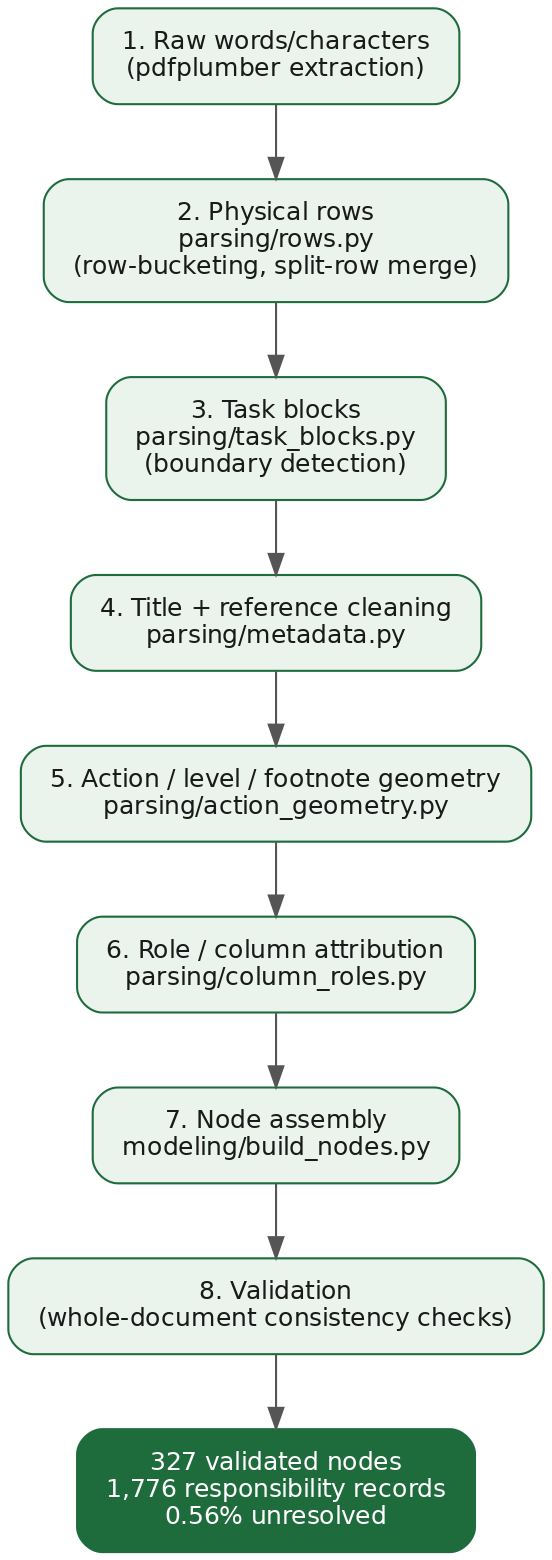
\includegraphics[width=0.82\textwidth,height=0.8\textheight,keepaspectratio]{figures/fig2_pipeline.png}
\caption{The eight-stage data engineering pipeline, from raw PDF extraction to a validated node set.}
\label{fig:pipeline}
\end{figure}

\begin{longtable}{|p{0.07\textwidth}|p{0.28\textwidth}|p{0.53\textwidth}|}
\caption{Stages of the data engineering pipeline.}\label{tab:stages}\\
\hline
\rowcolor{myblue}\textcolor{white}{\textbf{Stage}} & \textcolor{white}{\textbf{Name}} & \textcolor{white}{\textbf{Function}} \\
\hline
\endfirsthead
\hline
\rowcolor{myblue}\textcolor{white}{\textbf{Stage}} & \textcolor{white}{\textbf{Name}} & \textcolor{white}{\textbf{Function}} \\
\hline
\endhead
1 & Raw extraction & Characters and words with coordinates, fonts, and sizes are read from the PDF. \\ \hline
2 & Row reconstruction & Words are grouped into physical rows by vertical alignment, with split rows merged where the merge is provably safe. \\ \hline
3 & Task block detection & Rows are grouped into task blocks, and boundaries between consecutive activities are determined. \\ \hline
4 & Title and reference cleaning & Titles are normalised, cross-references are extracted and expanded, footnote digits are stripped from title text. \\ \hline
5 & Geometric attribution & Authority codes are separated from footnote markers by character geometry, and levels are attached. \\ \hline
6 & Role attribution & Codes are matched to roles by horizontal alignment with clustered, rotated column headers. \\ \hline
7 & Node assembly & Enriched blocks are validated against the schema and merged with the chapter and process skeleton. \\ \hline
8 & Validation & Whole-document consistency checks are run across the assembled node set. \\ \hline
\end{longtable}

\subsection{Data Flow and Modular Organisation}

Each stage lives in its own module, and the boundaries between them were drawn so that a failure can be localised by inspecting the output of one stage rather than by tracing execution through the whole program. During development this mattered constantly: when a record came out wrong, the question was always which stage first produced something incorrect, and that question is only cheap to answer if the intermediate results are inspectable.

Parsing modules handle rows, task blocks, metadata, action geometry, column roles, and text cleaning. Modelling modules handle node construction, the structural skeleton, the graph, and the cache. The schema sits in its own module, depended on by both groups and depending on neither.

\section{Data Ingestion}

Ingestion walks the document page by page. For each page, characters are read with their coordinates and font metrics, and words are read with their bounding boxes. Both are retained, since different stages need different granularity: row reconstruction works on words, while the superscript rule works on characters.

Reference data is ingested separately and from different pages of the same document. The authority code legend is transcribed into a structured file listing each full code, its level, and its meaning, and validated against the schema so that all seventeen entries load cleanly. The abbreviations pages are parsed into a glossary, which required its own handling: entries wrap across lines, some rows are section headings rather than definitions, and a term and its definition are occasionally rendered a fraction of a point out of alignment, so row grouping needs the same tolerance used elsewhere in the pipeline.

\section{Document Processing and Normalisation}

\subsection{Row Reconstruction}

Words are grouped into rows by clustering their vertical positions. A tolerance is applied, because text that is visually on the same line is frequently not at an identical coordinate. Where the Non-Sovereign Operations chapter splits a logical row into two bands, the two are merged under the restricted condition described in Chapter~2: only when the lower band consists entirely of authority codes.

\subsection{Task Block Detection}

Rows are then grouped into blocks, each corresponding to one activity. Boundary detection is the part of the pipeline that required the most iteration, because the visual cue for a boundary is inconsistent. Three signals are used together: whether a task is currently open, whether the open task's accumulated text ends with a full stop, and whether an incoming row carries authority codes when the open task already has some of its own. The third signal is the strongest, since a second batch of codes almost always indicates that the next activity has begun.

\subsection{Title and Reference Cleaning}

Titles are normalised by stripping footnote digits, collapsing whitespace, and removing cross-reference phrases that would otherwise be absorbed into the title as noise. Reference extraction is centralised in a single function used by every path that touches titles or notes. This was not the original design: two divergent implementations existed at one point, one of which handled a reference pattern the other did not, and the inconsistency produced titles that differed depending on which path had processed them.

\subsection{Geometric Attribution of Authority Codes}

Authority codes are identified within each row and separated from footnote markers by the character-level rule described in Chapter~2. Level digits belonging to a code are retained as part of it; superscript digits are recorded separately as footnote reference numbers attached to that responsibility.

\subsection{Role Attribution}

Role headers are extracted, clustered by horizontal position, and associated with the column region they label. Each authority code found in a row is then matched to the header cluster whose horizontal extent contains it. Where a page carries no headers because the table has continued from a previous page, the last seen header set is carried forward.

Roles that cannot be matched to any header are recorded as unresolved rather than discarded or guessed. Keeping them visible is deliberate: an unresolved role is a known gap that can be counted and reported, whereas a discarded one is an invisible loss.

\section{Node Construction and Validation}
\label{sec:nodeconstruction}

Enriched blocks are assembled into records conforming to the schema, and merged with a structural skeleton that supplies the chapter and process nodes, since those are organisational containers that the table parser never emits as activities.

Parentage is derived explicitly rather than inferred from identifier shape. Each record carries pointers to its parent, and the hierarchy is reconstructed from those pointers. An earlier implementation derived children by string prefix matching, which happens to work for two of the four levels and fails for the other two, and the failure was invisible until threshold variants entered the identifier space and a task's grandchildren began colliding with its direct children under the same prefix. The bug was caught by a consistency check requiring that every record's children be of the expected type and that every child's own parent pointer point back, rather than by inspection.

\begin{longtable}{|p{0.52\textwidth}|p{0.34\textwidth}|}
\caption{Data quality indicators after node construction.}\label{tab:quality}\\
\hline
\rowcolor{myblue}\textcolor{white}{\textbf{Indicator}} & \textcolor{white}{\textbf{Value}} \\
\hline
\endfirsthead
\hline
\rowcolor{myblue}\textcolor{white}{\textbf{Indicator}} & \textcolor{white}{\textbf{Value}} \\
\hline
\endhead
Structured records produced & 327 \\ \hline
Responsibility entries extracted & 1,776 \\ \hline
Distinct roles identified & 131 \\ \hline
Unresolved role entries & 10 (0.56\%) \\ \hline
Average responsibilities per record & 5.48 \\ \hline
Records with no direct responsibilities & 29.63\% \\ \hline
Cross-references captured & 14 \\ \hline
Responsibility entries carrying footnote references & 113 (6.36\%), across 44 records \\ \hline
Residual title corruption & 1 record (2.222.1) \\ \hline
\end{longtable}

\section{Knowledge Graph Modelling}

\subsection{Why a Graph}

The validated node set could have been stored as relational tables or as a flat document collection. A graph was chosen because the questions the system must answer are relationship questions. ``Who approves this activity'' is a traversal from an activity node along edges of a particular type, and ``which activities does this role approve'' is the same traversal in reverse. Both are single operations on a graph and joins or scans on a flat structure.

A directed multigraph is used rather than a simple graph, because a role can hold more than one distinct responsibility over the same activity. Two nodes may therefore be connected by several parallel edges, each carrying its own authority code and footnote references.

\subsection{Node and Edge Schema}

The graph contains two kinds of node. Activity nodes correspond one-to-one with the 327 structured records. Role nodes correspond to the 131 distinct roles. Edges carry the relationships between them.

\begin{longtable}{|p{0.24\textwidth}|p{0.24\textwidth}|p{0.42\textwidth}|}
\caption{Edge types in the knowledge graph.}\label{tab:edges}\\
\hline
\rowcolor{myblue}\textcolor{white}{\textbf{Edge type}} & \textcolor{white}{\textbf{From $\rightarrow$ To}} & \textcolor{white}{\textbf{Meaning}} \\
\hline
\endfirsthead
\hline
\rowcolor{myblue}\textcolor{white}{\textbf{Edge type}} & \textcolor{white}{\textbf{From $\rightarrow$ To}} & \textcolor{white}{\textbf{Meaning}} \\
\hline
\endhead
\texttt{contains} & Activity $\rightarrow$ Activity & Hierarchical containment: chapter to process, process to task, task to child task or threshold variant. \\ \hline
\texttt{responsible\_for} & Role $\rightarrow$ Activity & A recorded responsibility, carrying the authority code, its level, and any footnote references. \\ \hline
\texttt{references} & Activity $\rightarrow$ Activity & A cross-reference extracted from the activity's own text, including ranges expanded to their members. \\ \hline
\end{longtable}

\begin{figure}[htbp]
\centering
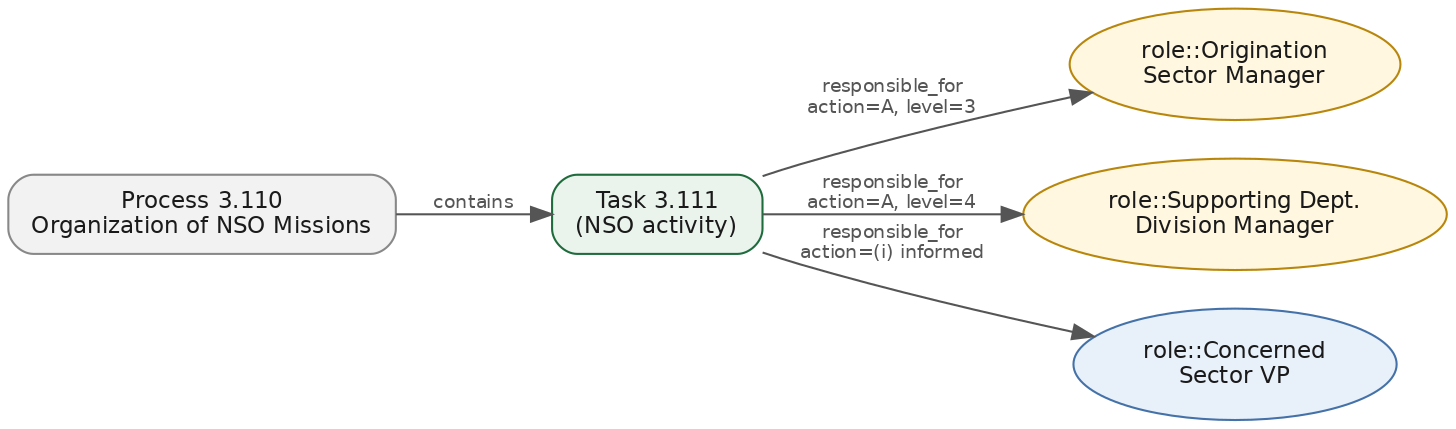
\includegraphics[width=0.82\textwidth,height=0.8\textheight,keepaspectratio]{figures/fig3_graph.png}
\caption{Excerpt of the knowledge graph around activity 3.111, showing the containment edge from its parent process and the responsibility edges connecting it to its approving and informed roles.}
\label{fig:graph}
\end{figure}

\subsection{Graph Statistics}

The assembled graph holds 459 nodes and 2,108 edges. The node count is the sum of the 327 activities and the 131 roles, plus one aggregate node. The edge count is dominated by responsibility edges, with containment edges accounting for the hierarchy and a small number of reference edges added from cross-references.

\section{Pipeline Evaluation}

\subsection{Execution and Caching}

A full rebuild from the PDF takes roughly fifteen to twenty seconds. That is acceptable offline and unacceptable per request, so the assembled node set is serialised to a cache file at build time and loaded at application startup. The running service never opens the PDF.

This was not the original arrangement, and the reason it changed is covered in Chapter~5: the first deployment attempt parsed the document during startup and was terminated by the hosting platform for exceeding its memory limit. Caching resolved that, and it also removed a subtler risk, since parsing at startup would have made the served content depend on the runtime environment rather than on a verified build artefact.

\subsection{Data Quality Outcomes}

The unresolved-role rate of 0.56 percent is the pipeline's headline quality figure, and it should be read carefully. It measures the proportion of extracted responsibility entries whose role could not be matched to a column header. It does not measure whether the correct code was extracted for every cell, which no automated check can establish in the absence of ground truth. That second question was addressed by sampling: specific activities were compared entry by entry against the printed page, including activities chosen precisely because they had previously been extracted incorrectly.

\subsection{Observed Limitations}

Two records in the processed subset, 2.516 and 2.522, have empty titles that the parser could not recover, and one record, 2.222.1, retains a residual title corruption. All three are known and documented rather than quietly accepted. A candidate fix for the last case was implemented, tested, found not to resolve the target case, found to introduce a regression elsewhere, and reverted. Leaving a documented defect in place was judged better than carrying a change that made the overall extraction worse.

A second limitation concerns footnotes and is discussed further in the general conclusion. Footnote reference numbers are extracted and attached to responsibilities, but the footnote text printed at the foot of each page is not yet parsed, so the system can report that a qualification applies without stating what it says. Two related extraction defects were identified during testing: on activities 1.116.1 and 1.116.2 a column header was mistaken for a role name, and on the same records two adjacent footnote digits were fused into a single number. Both are documented in Chapter~5 alongside the planned remediation.

The pipeline has also only been exercised against three chapters. The remaining chapters of the full document use the same table conventions as far as can be determined, but that expectation is untested, and processing them would be the first step of any continuation of this work.

\section*{Conclusion}
\addcontentsline{toc}{section}{Conclusion}

The pipeline converts a document whose structure is purely visual into 327 validated records carrying 1,776 responsibility entries, with under one percent of those entries unresolved, and turns that output into a graph of 459 nodes and 2,108 edges that answers relationship questions by traversal. Each stage is deterministic and inspectable, which is what allowed the defects described in Chapter~2 to be found, fixed, and prevented from recurring. The next chapter builds the agent that queries this graph.
